\chapter{Cahier des charges}
 
\section{Spécifications}
Les spécifications ont été choisi afin de satisfaire les donnés du cahier des charges (section \ref{cahierdescharges}).  La plupart des données étant plutôt vague, nous ont laissé encore une grande liberté de choix. 

\begin{table}[htbp]
    \centering
    \begin{tabular}{|c|c|c|}
        \hline
         & \textbf{Cahier des charges} & \textbf{Spécifications} \\
        \hline
        Dimensions & facile à transporter & trouver place sur une feuille A4 \\
        \hline
        Masse & facile à transporter & \SI{< 5}{\kilo\gram} \\
        \hline
        Temps & le plus cout possible & \SI{< 30}{\second} \\
        \hline
        Matériau & matériaux courants & aliage aluminium \\
        \hline
        Source d'énergie & manivelle & manivelle à petit rayon\\
        \hline
    \end{tabular}
    \caption{Les donnés du cahier des charges et les spécifications résultantes}
    %\label{tab:specifications1}
\end{table}

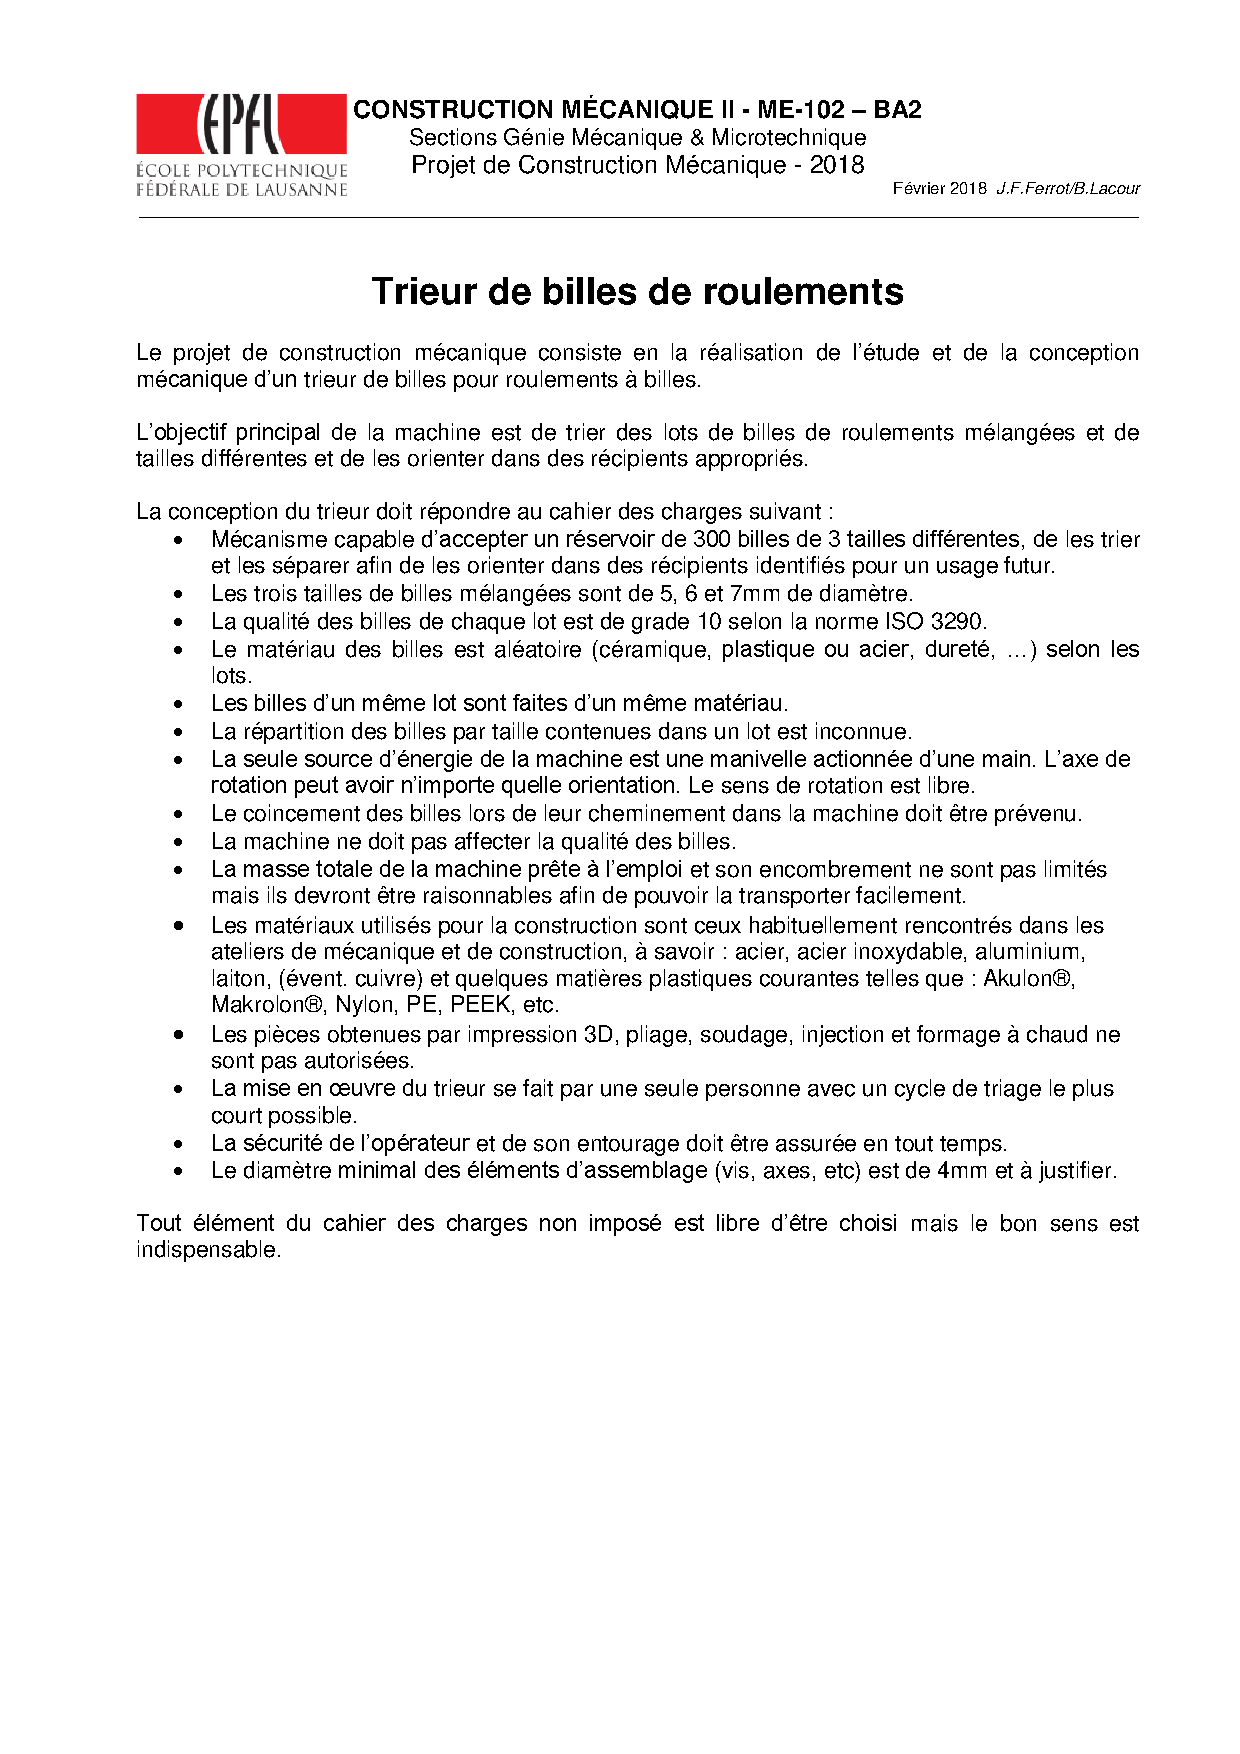
\includepdf[addtotoc={1,section,1,Cahier des charges donné,cahierdescharges}]{Documents/Cahier_de_charges.pdf}